\RequirePackage{flashmovie}
\documentclass[compress]{beamer}%

\mode<presentation>
{
%	\setbeamertemplate{background canvas}[vertical shading][bottom=red!10,top=blue!10]
%	\usetheme{Frankfurt}
%    \usetheme{Berkeley}
%    \usetheme{Madrid}
    \usetheme{Warsaw}
%    \usetheme{JuanLesPins}
%    \usefonttheme[stillsansserifmath]{serif}
	\usefonttheme[onlymath]{serif}
    \usecolortheme{default}
}
%\setbeamercolor{background canvas}{bg=black}
%\usepackage{amsmath,amssymb,amsthm,mathrsfs,amsfonts,dsfont}
\usepackage{dsfont}
\usepackage{epstopdf}
\usepackage{multirow}
%\usepackage{epsfig}
\usepackage{amssymb}
\usepackage{amsmath}
\usepackage[absolute,overlay]{textpos}
\usepackage{keyval}
\usepackage{units}
\usepackage{geometry}
\usepackage{tabu}
\usepackage{multimedia}
%\usepackage{movie15}
\usepackage{hyperref}
\usepackage{graphics,graphicx,subfigure}
\usepackage{caption}

%\usepackage{subcaption}
%\newcommand{\myurlshort}[2]{\href{#1}{\textcolor{gray}{\textsf{#2}}}}%\usepackage{wrapfig}
%\usepackage{pst-all}
\usepackage{media9}%


\newtheorem*{mydef}{Definition}
\newtheorem*{mythm}{Theorem}
%
%%*******Define Mathematical operators***************
%%The number e
%\providecommand*{\eu}%
%            {\ensuremath{\mathrm{e}}}
%%For setting units
\providecommand*{\unit}[1]{%
	\ensuremath{\mathrm{\,#1}}}

%differentiation
\makeatletter
\providecommand*{\diff}%
    {\@ifnextchar^{\DIfF}{\DIfF^{}}}
\def\DIfF^#1{%
    \mathop{\mathrm{\mathstrut d}}%
        \nolimits^{#1}\gobblespace}
\def\gobblespace{%
    \futurelet\diffarg\opspace}
\def\opspace{%
    \let\DiffSpace\!%
    \ifx\diffarg(%
        \let\DiffSpace\relax
    \else
        \ifx\diffarg[%
            \let\DiffSpace\relax
    \else
        \ifx\diffarg\{%
            \let\DiffSpace\relax
        \fi\fi\fi\DiffSpace}

\providecommand*{\deriv}[3][]{%
    \frac{\diff^{#1}#2}{\diff #3^{#1}}}

\providecommand*{\pderiv}[3][]{%
\frac{\partial^{#1}#2}%
{\partial #3^{#1}}}

\DeclareMathOperator{\St}{St}
\DeclareMathOperator{\diag}{diag}
%%
%%%
%\usepackage{media9}%
%\newcommand{\includemovie}[3]{%
%\includemedia[%
%width=#1,height=#2,%
%activate=pagevisible,%
%deactivate=pageclose,%
%addresource=#3,%
%flashvars={%
%src=#3 % same path as in addresource!
%&autoPlay=true % default: false; if =true, automatically starts playback after activation (see option ‘activation)’
%&loop=true % if loop=true, media is played in a loop
%&controlBarAutoHideTimeout=0 %  time span before auto-hide
%}%
%]{}{myPresentation.avi}%
%

\newcommand*{\vcenteredhbox}[1]{\begingroup
\setbox0=\hbox{#1}\parbox{\wd0}{\box0}\endgroup}
\newcommand{\thepic}{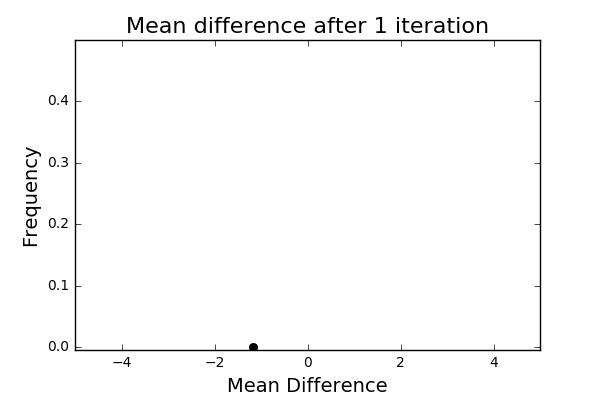
\includegraphics[width=5cm,height=5cm,keepaspectratio]{./figures/testp0.png}}
